\documentclass[../pbr.tex]{subfile}

\begin{document}
\section{Camera Projection}%
\label{sec:camera_projection}

The first stage of the rendering process is to project the rays from the
observer or camera. There are two types of projection, first Orthogonal
projection, and the Perspective projection. For the vast majority of
situations, the perspective projection is the projection method that will be
used, as it more accurately simulates cameras in reality. Because of this we do
not go into detail about the orthogonal projection method, nor has it been
implemented in Specula.

In more advance physically based renderer, camera lenses and the refractions
and effects caused by them are simulated as well. In our system we have not yet
implemented the lens system. This means that our camera simulates a pin hole
camera, and does not have a field of focus, or any of the features that one
would expect from a physical camera.

The model of the camera that we implement is a mirror of the physical pinhole
camera. I a pinhole camera, there is the pinhole aperture, and behind that
there is the plane of the film. Any of the light that passes through the
aperture is projected onto the film. Thus to project light going in the reverse
direction, we would consider each point on the film, and project a ray from
that point to the point of the pinhole. This process is depicted in Figure
\ref{fig:p1_pinhole1}.

\begin{figure}[htpb]
  \begin{center}
    \begin{minipage}{0.3\textwidth}
      \begin{center}
        \begin{tikzpicture}[scale=1, transform shape]
          \draw (-1.5,-1.0) -- (-1.5,1.0) node[above]{Film};
          \draw (0.0, -1.0) -- (0.0, -0.1);
          \draw (0.0, 0.1) -- (0.0, 1.0) node[above]{Aperture};
          \node at (1.5, 0.0)[fontscale=3] {\faTree};
          \node at (-1.5, 0.0)[fontscale=3,rotate=180] {\faTree};
          \draw[->] (-1.4,-1.0) -- (1.4,1.0);
          \draw[->] (-1.4,1.0) -- (1.4,-1.0);
        \end{tikzpicture}

        (a)
      \end{center}
    \end{minipage}
    \begin{minipage}{0.3\textwidth}
      \begin{center}
        \begin{tikzpicture}[scale=1, transform shape]
          \draw (1.5,-1.0) -- (1.5,1.0) node[above]{Film};
          \draw (0.0, -1.0) -- (0.0, -0.1);
          \draw (0.0, 0.1) -- (0.0, 1.0) node[above]{Aperture};
          \node at (3.0, 0.0)[fontscale=10] {\faTree};
          \node at (1.5, 0.0)[fontscale=1] {\faTree};
          \draw[->] (0,0) -- (3.0,2.0);
          \draw[->] (0,0) -- (3.0,-2.0);
        \end{tikzpicture}

        (b)
      \end{center}
    \end{minipage}
    \begin{minipage}{0.3\textwidth}
      \begin{center}
        \begin{tikzpicture}[scale=1, transform shape]
          \draw (3.0,-1.0) -- (3.0,1.0) node[above]{Film};
          \draw (0.0, -1.0) -- (0.0, -0.1);
          \draw (0.0, 0.1) -- (0.0, 1.0) node[above]{Aperture};
          \node at (1.5, 0.0)[fontscale=1] {\faTree};
          \node at (3.0, 0.0)[fontscale=4] {\faTree};
          \draw[->] (0,0) -- (3.0,1.0);
          \draw[->] (0,0) -- (3.0,-1.0);
        \end{tikzpicture}

        (c)
      \end{center}
    \end{minipage}
  \end{center}
  \caption{A standard pinhole camera(a) produces a flipped image, our camera
    (b) and (c) produces a upright image, which is proportionally scaled to the
    scene.}%
  \label{fig:p1_pinhole1}
\end{figure}

Because of the digital nature of the system, we are able to develop some slight
alternatives to the pinhole camera, which are simpler and more efficient to
implement. These alternatives are based on moving the plane of the film to be
in front of the aperture, in stead of behind it. The distance of the film from
the aperture adjusts the field of view of the image. For example if the plane
of the film is close to the aperture, then the result would relate to a large
field of view, and this case is demonstrated in Figure
\ref{fig:p1_pinhole1}.(b). Then if the field of view is small, this would
relate to the film plane being very far away from the plane of the aperture,
and this is also demonstrated in Figure \ref{fig:p1_pinhole1}.(c). This process
can be described as selected a point on the film, and projecting the ray of
light from the aperture, through this point on the film, and further into the
scene.

\subsection{Film}%
\label{sub:film}

For the purposes of generating an image, we will consider the film to be
constructed of discrete pixels. By determining the color of each pixel, we can
then generate the output image. The data for each pixel will be computed by the
path marching process, and then stored in the film object. Once all pixels have
been colors, it is then possible to output the film into any common image
format. Specula implements generating \texttt{png}, \texttt{jpeg}, and
\texttt{bmp} images.

\subsection{Sampling}%
\label{sub:sampling}

As described previously, the primary process used for determining the colors of
the pixels on the film, is to project a ray from the aperture through the film
and then into the scene. To do this we must determine which point on the film
to project rays of light though.

The naive method to do this, is to send a single ray through the center of each
pixel of the film. This will produce acceptable results, but it has some
problems. Consider a pixel as shown in Figure \ref{fig:p1_pixel}.(a). This pixel
using this method would be grey, the color of the circle. However, that is
loosing about $21\%$ of the data in the pixel, all of the white space is being
forgotten about, and in this case that accounts for approximately $21\%$ of the
pixel, but there are other cases where it could account for more, like in
Figure \ref{fig:p1_pixel}.(b), the center pixel will be considered to be grey,
but by far the majority of the pixel is white, in this case $87\%$ of the data
present in that pixel is being lost.

\begin{figure}[htpb]
  \begin{center}
    \begin{minipage}{0.45\textwidth}
      \begin{center}
        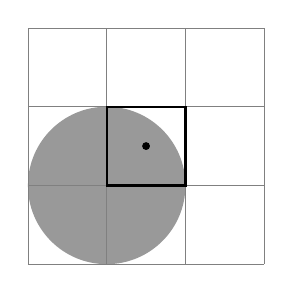
\begin{tikzpicture}[scale=1, transform shape]
          \fill[black!40!white] (1,1) circle (1.0);
          \draw[step=1,gray,very thin] (0,0) grid (3,3);
          \draw[thick] (1,1) rectangle (2,2);
          \fill (1.5,1.5) circle(0.05);
        \end{tikzpicture}

        (a)
      \end{center}
    \end{minipage}
    \begin{minipage}{0.45\textwidth}
      \begin{center}
        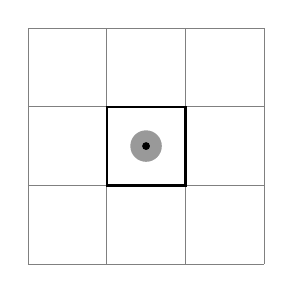
\begin{tikzpicture}[scale=1, transform shape]
          \fill[black!40!white] (1.5,1.5) circle (0.2);
          \draw[step=1,gray,very thin] (0,0) grid (3,3);
          \draw[thick] (1,1) rectangle (2,2);
          \fill (1.5,1.5) circle(0.05);
        \end{tikzpicture}

        (b)
      \end{center}
    \end{minipage}
  \end{center}
  \caption{Pixel with multiple possibilities}%
  \label{fig:p1_pixel}
\end{figure}

The method that we implement to resolve this issue, is to sample multiple rays
for each pixel in the image, where each ray is at a different random location
in the pixel. The points in each pixel are uniformly distributed over the area,
and thus as the number of samples per pixel(\textit{spp}) approaches infinity,
then the average color of these rays represents the average color of the pixel
as a whole.

Considering our examples from before, but by taking multiple
samples we preserve more information present in the pixel. In Figure
\ref{fig:p1_spp_pixel}.(a), we find that the pixel should be $75\%$ grey, and
$25\%$ white. While not the exact value that the color should be, it is a much
better representation than a single sample would provide us. In Figure
\ref{fig:p1_spp_pixel}.(b), we find that the pixel should be $50\%$ grey, and
$50\%$ white. Again, not the exact value that we would expect, but it is
significantly better. Both of these examples have only been computed with four
samples, and the rendering system will generally sample each pixel in the range
of $128-4096$, but the user is able to adjust this to be higher or lower as
desired.

\begin{figure}[htpb]
  \begin{center}
    \begin{minipage}{0.45\textwidth}
      \begin{center}
        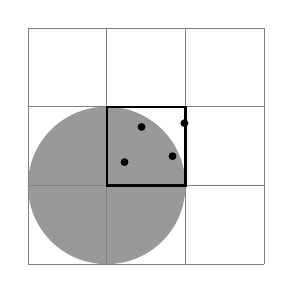
\begin{tikzpicture}[scale=1, transform shape]
          \fill[black!40!white] (1,1) circle (1.0);
          \draw[step=1,gray,very thin] (0,0) grid (3,3);
          \draw[thick] (1,1) rectangle (2,2);
          \fill (1.836,1.371) circle(0.05); % GREY
          \fill (1.987,1.791) circle(0.05); % WHITE
          \fill (1.442,1.743) circle(0.05); % GREY
          \fill (1.226,1.296) circle(0.05); % GREY
        \end{tikzpicture}

        (a)
      \end{center}
    \end{minipage}
    \begin{minipage}{0.45\textwidth}
      \begin{center}
        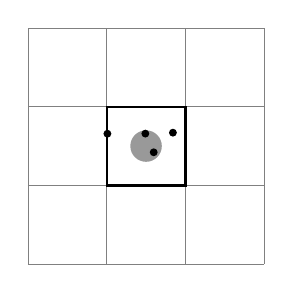
\begin{tikzpicture}[scale=1, transform shape]
          \fill[black!40!white] (1.5,1.5) circle (0.2);
          \draw[step=1,gray,very thin] (0,0) grid (3,3);
          \draw[thick] (1,1) rectangle (2,2);
          \fill (1.009,1.657) circle(0.05); % WHITE
          \fill (1.597,1.421) circle(0.05); % GREY
          \fill (1.841,1.670) circle(0.05); % WHITE
          \fill (1.491,1.658) circle(0.05); % GREY
        \end{tikzpicture}

        (b)
      \end{center}
    \end{minipage}
  \end{center}
  \caption{Pixel with with multiple random samples}%
  \label{fig:p1_spp_pixel}
\end{figure}

Intuitively this is clear that with more samples, the approximation of the
color within the pixel becomes more accurate. We verify this using a numeric
simulation of the example in Figure \ref{fig:p1_spp_pixel}.(b). It is clear
that this process is equivalent to approximating the area of the shaded region
within the pixel. So we developed a script to randomly sample points within the
pixel to approximate the area of the shaded circle. The resulting plot of the
approximated area, and the error of that approximation is shown in Figure
\ref{fig:p1_spp_approx}.

\begin{figure}[htpb]
  \begin{center}
    \begin{tikzpicture}[scale=1, transform shape]
      \begin{axis}
        \addplot[blue] table [x=spp, y=approx, col sep=comma] {./scripts/spp_proof.csv};
        \addplot[red] table [x=spp, y=error, col sep=comma] {./scripts/spp_proof.csv};
        \legend{Approx,Error};
      \end{axis}
    \end{tikzpicture}
  \end{center}
  \caption{Convergence of approximation and error for pixel sampling}%
  \label{fig:p1_spp_approx}
\end{figure}

This will be our method for the initial sampling of rays from the camera into
the scene, each ray which we sample will return a color. Each ray within a
pixel will be averaged and the average color will be used for the color of the
pixel.

\end{document}
